% Name: Minimax game tree
% Description: A two-ply game tree: MIN takes the smallest leaf below each move, MAX takes the largest of those, and the best move is highlighted.
% Tags: minimax, game tree, adversarial search, artificial intelligence

\usetikzlibrary{shapes.geometric}

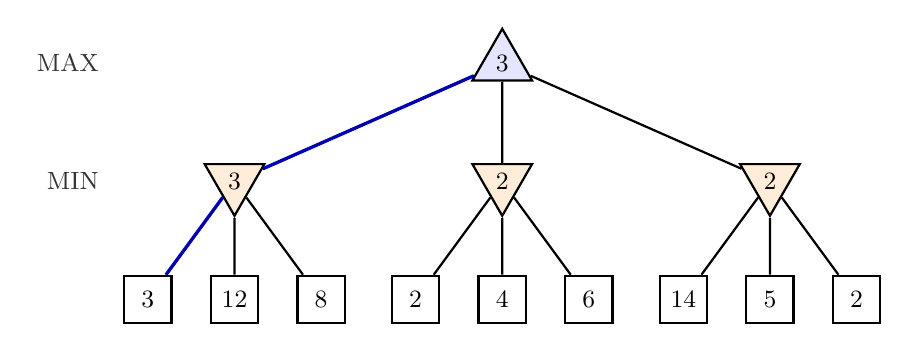
\begin{tikzpicture}[
  level distance=15mm,
  level 1/.style={sibling distance=34mm},
  level 2/.style={sibling distance=11mm},
  every node/.style={font=\small},
  max/.style={regular polygon, regular polygon sides=3, draw, thick, inner sep=1.5pt, fill=blue!10},
  min/.style={max, shape border rotate=180, fill=orange!15},
  leaf/.style={draw, thick, minimum size=6mm},
  edge from parent/.style={draw, thick},
]
  % MIN values: min(3,12,8) = 3, min(2,4,6) = 2, min(14,5,2) = 2; MAX value: max(3,2,2) = 3
  \node[max] (root) {3}
    child { node[min] (move) {3}
      child { node[leaf] (leaf) {3} } child { node[leaf] {12} } child { node[leaf] {8} } }
    child { node[min] {2}
      child { node[leaf] {2} } child { node[leaf] {4} } child { node[leaf] {6} } }
    child { node[min] {2}
      child { node[leaf] {14} } child { node[leaf] {5} } child { node[leaf] {2} } };
  % The best move and the leaf value it leads to
  \draw[very thick, blue!70!black] (root) -- (move) -- (leaf);
  \node[anchor=east, gray!40!black] at (-5,0) {MAX};
  \node[anchor=east, gray!40!black] at (-5,-1.5) {MIN};
\end{tikzpicture}
